\part{Physische Datenspeicherung}
\section{Speichersysteme}

\subsection{Speicherhierarchie}

\begin{frame}
	\frametitle{\insertsection}
	\framesubtitle{\insertsubsection}
	\begin{figure}
		\includegraphics[scale=0.36]{img/memhierarchyPlus.png}
		\caption{Speicherhierarchie (Quelle: \cite[S. 432]{SKS11})}
	\end{figure}
\end{frame}

\begin{frame}
	\frametitle{\insertsection}
	\framesubtitle{\insertsubsection}
    \structure{Generell gilt: Je schneller, desto kleiner und teurer.\abs Standard-Speicherhierarchie:}
    \begin{itemize}
        \item Cache
        \begin{itemize}
            \item Direkt an der CPU
            \item Normalerweise verwendet für Pipelining und Prefetching
        \end{itemize}
        \pause
        \item Hauptspeicher
        \begin{itemize}
            \item Heute im Bereich zwischen 4-32 GB (Standard) oder 128 GB bis 6 TB (In-Memory-DB)
            \item In-Memory DB: Komplette Datenbanken im Hauptspeicher
        \end{itemize}
        \pause
        \item Festplattensysteme 
        \begin{itemize}
            \item Speicherkapazität im Terabyte-Bereich
            \item Können im Verbund Petabytes an Daten speichern
            \item Faktor Zugriffszeit (magnetische Festplatte -- Memory): $100.000$
        \end{itemize}
    \end{itemize}
\end{frame}

\begin{frame}
	\frametitle{\insertsection}
	\framesubtitle{\insertsubsection}
    \structure{Datenbanken speichern die Daten persistent, d.h. permanent auf einer Festplatte:}\\[6pt]
    \begin{itemize}
        \item Die meisten Datenbanken sind zu groß, um sie im Hauptspeicher zu halten.\\[4pt]
        \item Primärer Speicher ist ausfallgefährdeter als sekundärer Speicher.\\[4pt]
        \item Kosten für Sekundärspeicher deutlich geringer als f\"ur Prim\"arspeicher.\\[4pt]
        \item Auch In-Memory-Datenbanken persistieren die Daten regelm\"a\ss ig auf Festplatten.
    \end{itemize}
\pause
\abs
Im Rahmen dieser Vorlesung:
\nl
Datenbanken werden in der Regel auf Festplattensystemen gespeichert.
\end{frame}

\subsection{Arbeitsweise}

\begin{frame}
\frametitle{\insertsection}
\framesubtitle{\insertsubsection}
\structure{Aufbau einer Festplatte}
\begin{columns}
	\begin{column}{.48\textwidth}
		\begin{figure}
			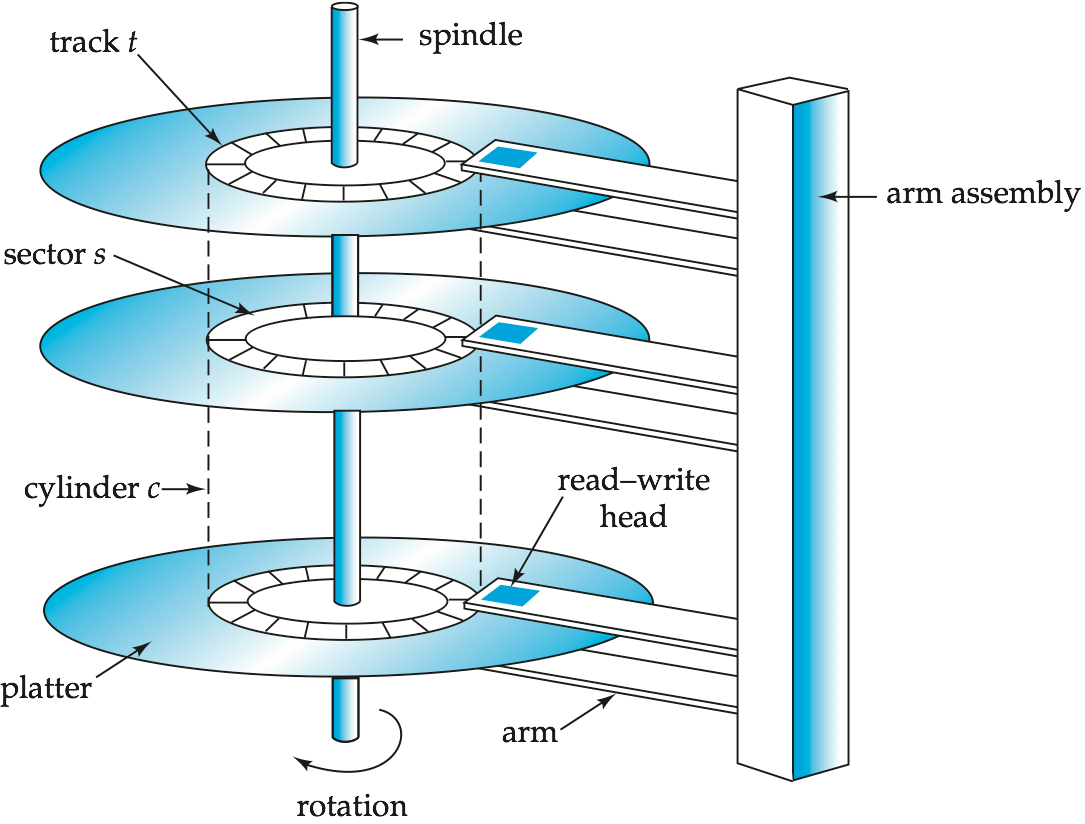
\includegraphics[scale=0.35]{img/hdd.png}
			\caption{Festplatte: Schematischer Aufbau (Quelle: \cite[S. 433]{SKS11})}
		\end{figure}
	\end{column}
	\begin{column}{.5\textwidth}
		\begin{itemize}
			\item Festplatten sind meist in mehrere einzelne Magnetplatten unterteilt
			\item Ein Zugriffsarm für jede Platte
			\item Platten sind in Spuren (Tracks) unterteilt
			\item Spuren sind in Sektoren oder Datenbl\"ocke unterteilt
			\item	Datenbl\"ocke bilden kleinste Zugriffseinheit auf der Festplatte
			\item Vertikal gestapelte Spuren hei\ss en Zylinder
		\end{itemize}
		\vspace{4em}
	\end{column}
\end{columns}
\end{frame}

\begin{frame}
\frametitle{\insertsection}
\framesubtitle{\insertsubsection}
\structure{Zugriff auf die Daten einer Festplatte}
\\[4pt]
\begin{itemize}
	\item Mittlere Zugriffszeit
	\begin{itemize}
		\item Seek Time (Schreib-Lese-Kopf in Position bringen): 6-8ms
		\item Latency (Warten, bis der richtige Sektor den Kopf passiert): 2-3ms
		\item Transferzeit (Daten von Platte in den Speicher übertragen): 15 MB/s
	\end{itemize}
	\pause
	\abs      				
	\item Daten werden \textbf{blockweise} in Hauptspeicher übertragen.
	\begin{itemize}
		\item G\"angig sind Bl\"ocke mit Gr\"o\ss en von 512 Bytes bis 8 KB.
		\item Suchen des ersten Blocks auf Platte dauert lange (\textit{SeekTime + Latency})
		\item Sind Bl"ocke konsekutiv angeordnet, k\"onnen Folgebl\"ocke direkt gelesen werden
		\item Sind Bl\"ocke nicht konsekutiv angeordnet: \textit{SeekTime + Latency} f\"ur jeden weiteren Block 
	\end{itemize}
\end{itemize}
\abs
\pause
\alert{Festplattenzugriffe / Anzahl der \textbf{Blockzugriffe} sind \textbf{teuer} und m\"ussen minimiert werden!}
\end{frame}

\section{Seiten und Datens\"atze}

\subsection{Grundlegende Betrachtungen}

\begin{frame}
\frametitle{\insertsection}
\framesubtitle{\insertsubsection}
\textbf{Seite = Dateneinheit im Speicher}
\begin{itemize}
	\item Die kleinste Dateneinheit im Speicher eines Datenbanksystems sind \textbf{Seiten}.
	\begin{itemize}
		\item Eine Seite umfasst mehrere Bl\"ocke, die in der Regel in einer Spur liegen.
	\end{itemize}
	\item Jede Relation wird in mehreren Seiten im Speicher gespeichert.
\end{itemize}
\pause
\ \\[20pt]
\textbf{Datensatz (Record) = Abbildung des logischen Tupels einer Relation im Speicher}
\begin{itemize}
	\item Ein Tupel der Relation wird in einem \textbf{Datensatz} gespeichert.
	\item Der Datensatz liegt in einer Seite und geht nicht \"uber Seitengrenzen hinaus.
	\item Ein oder mehrere Datens\"atze können in einer Seite abgelegt werden.
\end{itemize}
\end{frame}

\begin{frame}
\frametitle{\insertsection}
\framesubtitle{\insertsubsection}
\structure{Speicherung einer Relation in Seiten und Datens\"atze}
\begin{columns}	
\begin{column}{.3\textwidth}
	\begin{tabular}{|c|c|c|}\hline
		\multicolumn{3}{|c|}{\small \textbf{\texttt{Vorlesungen}}}\\\hline\hline
		\small \textbf{{\texttt{VID}}} & \small \textbf{{\texttt{Name}}} & \small \textbf{{\texttt{\ldots}}}\\\hline 
		\small 5001 & \small Grundz\"uge & \small \ldots\\\hline 
		\small 4052 & \small Logik & \small \ldots\\\hline 
		\small 5041 & \small Ethik  & \small \ldots\\\hline 
		\small \ldots & \small \ldots & \small \ldots\\\hline 
	\end{tabular}
	\hspace{3mm}
\end{column}
\begin{column}{.48\textwidth}
	\begin{figure}
		\includegraphics[scale=0.3]{img/Seite-4711-2.png}
		\caption{Seiten mit Datens\"atzen}
	\end{figure}
\end{column}\end{columns}
\end{frame}

\begin{frame}
\frametitle{\insertsection}
\framesubtitle{\insertsubsection}
\structure{Alle I/O-Operationen der Datenbank durchlaufen den Datenbankpuffer}
\begin{itemize}
	\item Datenbankpuffer ist Teil des Hauptspeichers, der (tempor\"ar) Kopien der Seiten speichert.
	\pause
	\abs
	\item Daten der Relationen werden seitenweise von der Festplatte gelesen und auf \textit{Seiten} im Puffer geschrieben. 
	\item \textbf{DB-Operationen erfolgen ausschlie\ss lich auf den Datens\"atzen im Puffer}.
	\item Die Daten werden erst \textbf{nach Abschluss aller relevanten Operationen} auf die Festplatte zur\"uckgeschrieben.\\[6pt]
	\pause
	\abs
	\item Die Verwaltung des Puffers beinhaltet:
	\begin{itemize}
		\item Speicherreservierung und Speicherfreigabe
		\item Suchen, Ersetzen/Swapping von Seiten im Puffer
		\item Synchronisation der Pufferseiten -- im Multiuser- und Multiprogramming-Betrieb wichtig
	\end{itemize}
\end{itemize}    
\end{frame}

\begin{frame}
\frametitle{\insertsection}
\framesubtitle{\insertsubsection}
\begin{figure}
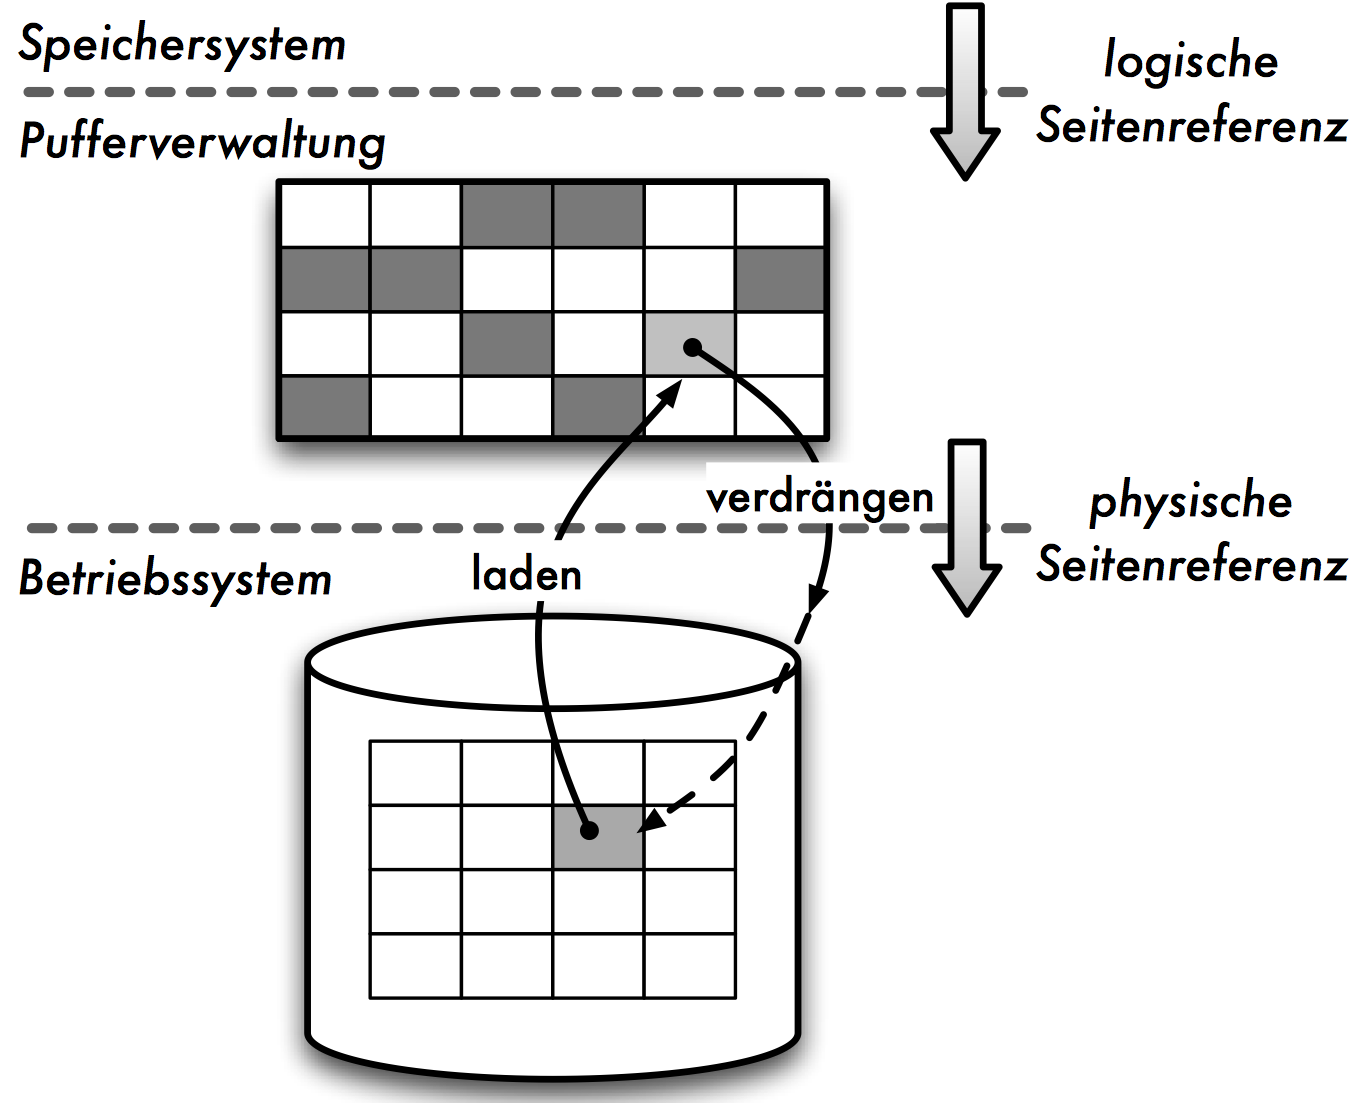
\includegraphics[scale=0.13]{img/buffer.png}
\caption{Zugriff auf Seite über Pufferverwaltung (Quelle: \cite[S. 31]{SSH11})}
\end{figure}
\end{frame}

\subsection{Aufbau eines Datensatzes}

\begin{frame}
\frametitle{\insertsection}
\framesubtitle{\insertsubsection}
\textbf{Felder eines Datensatzes}
\begin{itemize} 
	\item Ein Datensatz ist eine Sammlung von \textbf{Feldern}.
  \item Zu jedem Attribut eines Tupels einer Relation geh\"ort ein Feld des Datensatzes.
	% \item Ein Record ist eine Kollektion von Feldern, die in einer Beziehung zueinander stehen	
	\item Ein Feld speichert den Wert des entsprechenden Attributs des Tupels.\\[20pt]
	\item Jedes Feld wird durch ein oder mehrere Bytes repräsentiert.
	\item Die Felder sind typisiert (\texttt{bool, int} etc.).
  %	\item Alle Felder und ihre zugehörigen Datentypen bestimmen den Recordtyp
	\pause
	\item Zu gro\ss e Attributwerte (z.~B.~Bilder) werden i.~d.~R.~ausgelagert:
	\begin{itemize}
		\item Daf\"ur existieren spezielle Datentypen:
		\begin{itemize}
			\item Binary Large Object (\texttt{BLOB}) für Binärdaten (Bilder, Musik etc.)
			\item Character Large Object (\texttt{CLOB}) für Textdaten (Fliesstexte, Webseiten etc.)
		\end{itemize}  
		\item Es wird nur eine Referenz (Pointer) im Feld gespeichert
		\item Die Daten selbst werden aus der Seite ausgelagert
	\end{itemize}	
\end{itemize}
\end{frame}

\begin{frame}
	\frametitle{\insertsection}
	\framesubtitle{\insertsubsection}
 \begin{itemize}
	\item Datens\"atze werden durch folgende Typen klassifiziert:
	\begin{itemize}
		\item 'Fixed Length Records' oder 'Fixl\"angen-Speicherung': Datens\"atze haben immer die gleiche L\"ange, auch wenn reservierter 
		Speicher ggf.~nicht verwendet wird.
		\item 'Variable Length Records' oder 'Speicherung in variabler L\"ange': Datens\"atze belegen nur den tats\"achlich verwendeten 
		Speicher.
	\end{itemize}
\end{itemize}    
\end{frame}

\begin{frame}[fragile]
	\frametitle{\insertsection}
	\framesubtitle{\insertsubsection}
\begin{columns}
\begin{column}{.48\textwidth}
    \structure{Struktur eines Fix-Length-Datensatzes}
    \lstset{language=c}
    \begin{lstlisting}[xleftmargin=3ex]
struct mitarbeiter {
  char name[30];
  char ssn[9];
  int salary;
  int job_code;
  char department[20];
} ;
    \end{lstlisting}
\end{column}
\begin{column}{.48\textwidth}
    \structure{Struktur eines Variable-Length-Datensatzes}
    \lstset{language=C}
    \begin{lstlisting}[xleftmargin=3ex]
struct mitarbeiter {
  char* name; /* Pointer */
  char ssn[9];
  int salary;
  int job_code;
  char* department /* Pointer */;
} ;
    \end{lstlisting}
\end{column}
\end{columns}
\end{frame}

\subsection{Abbildung im Hauptspeicher}

\begin{frame}
	\frametitle{\insertsection}
	\framesubtitle{\insertsubsection}
	\structure{Fixl\"angen-Speicherung}
	\begin{itemize}
		\item F\"ur jedes Feld wird im Speicher eine feste Anzahl von Bytes reserviert 
		\item Vorteil: Sehr einfache und schnelle Adressierung
		\item Nachteil: Unflexibel bez\"uglich \"Anderung der Datengr\"o\ss e
	\end{itemize}	
	 \begin{figure}
	 	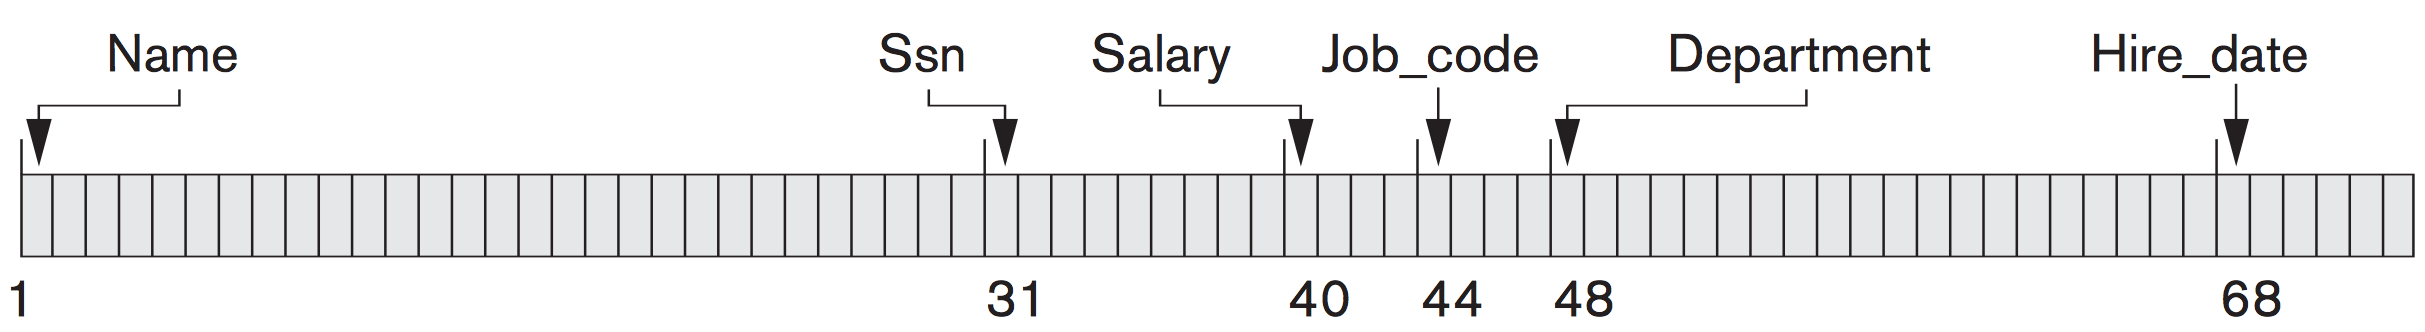
\includegraphics[scale=0.13]{img/fix.png}
	 	\caption{Fixlängen-Speicherung (Quelle: \cite[S. 596]{EN10})}
	 \end{figure}
\end{frame}

\begin{frame}
	\frametitle{\insertsection}
	\framesubtitle{\insertsubsection}
	\structure{Speicherung in variabler L\"ange -- Alternative 1}
	\begin{itemize}
		\item Zwischen Feldern variabler L\"ange wird ein spezielles Trennzeichen gesetzt. 
		\item Vorteil: Keine Speicherplatzverschwendung und flexibel bez\"uglich Datengr\"o\ss e.
		\item Nachteil: Langsamerer Zugriff als bei Fixl\"angen.
	\end{itemize}	
	\begin{figure}
		\includegraphics[scale=0.13]{img/var.png}
		\caption{Speicherung in variabler L\"ange -- Alternative 1 (Quelle: \cite[S. 596]{EN10})}
	\end{figure}
\end{frame}

\begin{frame}
	\frametitle{\insertsection}
	\framesubtitle{\insertsubsection}
	\structure{Speicherung in variabler L\"ange -- Alternative 2}
	\begin{itemize}
		\item Speicherung als Key-Value-Paare
		\item Nicht gesetzte Felder werden nicht mehr explizit gespeichert. 
		\item Vorteil: Es wird nur noch der minimal notwendige Speicherplatz belegt.
		\item Nachteil: Auslesen der Key-Value-Paare aufw\"andig.
	\end{itemize}
	\begin{figure}
		\includegraphics[scale=0.13]{img/var2.png}
		\caption{Speicherung in variabler L\"ange, Alternative 2 (Quelle: \cite[S. 596]{EN10})}
	\end{figure}
\end{frame}

\subsection{Abbildung im Hauptspeicher -- Dateien und Bl\"ocke}

\begin{frame}
	\frametitle{\insertsection}
	\framesubtitle{\insertsubsection}
    \structure{Organisationsformen \textit{Unspanned} und \textit{Spanned}}
    \begin{itemize}
    	\item DB-Dateien bestehen aus Sequenzen von Datens\"atzen: Datens\"atze werden in Dateien geschrieben.
      \item Datens\"atze innerhalb einer Datei sind (normalerweise) vom gleichen Relationentyp.
      \pause
      \item Die Datens\"atze werden in einer Datei in Bl\"ocken im Unspanned- bzw.~im Spanned-Modus gespeichert ...
    \end{itemize}
\end{frame}

\begin{frame}
\frametitle{\insertsection}
\framesubtitle{\insertsubsection}
\structure{Organisationsformen \textit{Unspanned} und \textit{Spanned}}
\abs
\emph{Unspanned}: Pro Block werden nur ein oder mehrere vollst\"andige Datens\"atze gespeichert
	\begin{itemize}
		\item Ungenutzter Speicherplatz am Ende eines Blocks
	\end{itemize}
  \begin{figure}
	 \includegraphics[width=200pt]{img/unspanned.png}
	 \caption{Unspanned (Quelle: \cite[S. 598]{EN10})}
  \end{figure}
\end{frame}


\begin{frame}
\frametitle{\insertsection}
\framesubtitle{\insertsubsection}
\structure{Organisationsformen \textit{Unspanned} und \textit{Spanned}}
\abs
\emph{Spanned}: Es können auch nur Teile eines Datensatzes in einem Block gespeichert werden. 
	\begin{itemize}
		\item Am Ende eines Blocks wird ein Pointer auf den nachfolgenden Block gesetzt.
		\item Ein Datensatz kann sich \"uber mehrere Bl\"ocke '\textit{spannen}'.
		\item Stets zu verwenden, wenn die Datens\"atze gr\"o\ss er als die Bl\"ocke sind. 
	\end{itemize}
  \begin{figure}
 	 \includegraphics[width=200pt]{img/spanned.png}
	 \caption{Spanned (Quelle: \cite[S. 598]{EN10})}
  \end{figure}
\end{frame}

\begin{frame}
\frametitle{\insertsection}
\framesubtitle{\insertsubsection}
\begin{definition}[Blocking Factor]
	Für gegebene effektive Blockgr\"o\ss e $B$ und L\"ange der Datens\"atze $R$ ist der Blocking Factor gegeben durch:
	$$bfr = \left \lfloor \frac{B}{R}\right \rfloor$$
\end{definition}
\pause
\ \\[-18pt]
\begin{block}{\textbf{Bemerkung}}
	\begin{itemize}
		\item \textit{bfr} gibt maximale Anzahl vollst\"andiger Datens\"atze pro Block an.
		\item In der Organisationsform 'Unspanned' bleiben $B-(bfr \cdot R)$ Bytes pro Block ungenutzt, und es werden
		$\left \lceil \frac{n}{bfr}\right \rceil$ Bl\"ocke für die Speicherung von $n$ Datens\"atzen ben\"otigt. \textbf{Warum?}
	\end{itemize} 
\end{block}
\pause
\ \\[-8pt]
\textbf{Beispiel:}
$B=512,\ R=120 \Rightarrow bfr = \left\lfloor\frac{512}{120}\right\rfloor = 4$. Im Unspanned-Modus
bleiben somit $512-(4 \cdot 120)=32$ Bytes pro Block ungenutzt. F\"ur $n=250$ Datens\"atze werden 
dann $\left \lceil \frac{250}{4}\right \rceil = 63$ Bl\"ocke ben\"otigt.
\end{frame}

\subsection{Speicherung von Dateien}

\begin{frame}
\frametitle{\insertsection}
\framesubtitle{\insertsubsection}
\structure{Verschiedene Verfahren zur Speicherung zusammengeh\"orender Bl\"ocke auf der Festplatte:}
\abs
\textbf{Contiguous Allocation}
	\begin{itemize}
		\item Alle Bl\"ocke werden konsekutiv hintereinander geschrieben
		\item Vorteil: Hohe Lesegeschwindigkeit
		\item Nachteil: Teure Einf\"ugeoperationen
	\end{itemize}\ \\[4pt]
\begin{figure}
	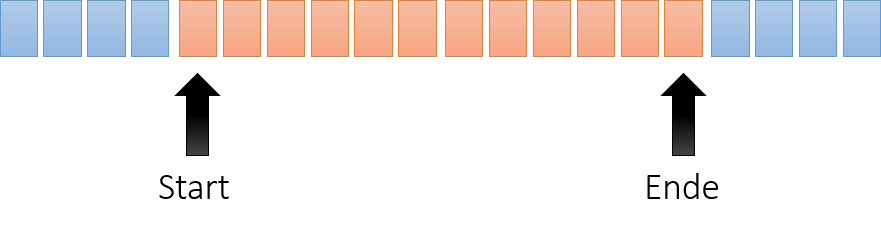
\includegraphics[width=200pt]{img/cont.png}
\end{figure}
\end{frame}

\begin{frame}
\frametitle{\insertsection}
\framesubtitle{\insertsubsection}
\structure{Verschiedene Verfahren zur Speicherung zusammengeh\"orender Bl\"ocke auf der Festplatte}
\abs
\textbf{Linked Allocation}
	\begin{itemize}
		\item Am Ende jedes Blocks befindet sich ein Pointer auf den n\"achsten Block
		\item Vorteil: Einf\"ugeoperationen problemlos realisierbar
		\item Nachteil: Teure Leseoperationen
	\end{itemize}\ \\[4pt]
\begin{figure}
	\includegraphics[width=200pt]{img/linked.png}
\end{figure}
\end{frame}

\begin{frame}
\frametitle{\insertsection}
\framesubtitle{\insertsubsection}
\structure{Verschiedene Verfahren zur Speicherung zusammengeh\"orender Bl\"ocke auf der Festplatte}
\abs
\textbf{Clustered Allocation}
	\begin{itemize}
		\item Konsekutive Block-Cluster werden untereinander verlinkt
		\item Kompromissl\"osung zwischen Contiguous Allocation und Linked Allocation
	\end{itemize}
\begin{figure}
	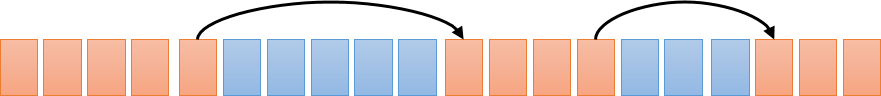
\includegraphics[width=200pt]{img/clustered.png}
\end{figure}
\end{frame}

\section{Formen der Dateiorganisation}
\subsection{Heap-Dateien}

\begin{frame}
	\frametitle{\insertsection}
	\framesubtitle{\insertsubsection}
	\structure{\textbf{Heap-Dateien}}\\[4pt]
	\begin{itemize}
		\item In einer Heap-Datei werden die Datens\"atze unsortiert sequentiell auf dem Datenträger gespeichert.\\[4pt]
		\item Neue Einträge werden ans Ende der Datei angeh\"angt. Stichwort: \textit{append}-Operation.\\[4pt]
		\item Die Adresse des letzten Blocks/der letzten Seite der Datei ist im Datei-Header abgespeichert.
	\end{itemize}	
\end{frame}

\begin{frame}
\frametitle{\insertsection}
\framesubtitle{\insertsubsection}
\structure{\textbf{Einf\"ugen in einer Heap-Datei}}	
\begin{itemize}
	\item Erster Datei-Block wird in den Hauptspeicher geladen.\\[4pt]
	\item Aus den Header-Informationen wird der letzte Block der Datei identifiziert.\\[4pt]
	\item Letzter Block der Datei wird in den Hauptspeicher geladen. \\[4pt]
	\item Ein neuer Datensatz wird in den letzten Block geschrieben. \\[4pt]
	\item Falls nicht mehr genug Platz im letzten Block vorhanden ist, wird ein neuer Block erzeugt.\\[4pt]
	\item Block wird auf Platte zur\"uck geschrieben -- ggf.~Update der Adresse des letzten Blocks im Header.\\[4pt]
\end{itemize}
\pause
Fazit: Einf\"uge-Operationen sehr effizient, da immer nur am Ende angeh\"angt wird.
\end{frame}

\begin{frame}
\frametitle{\insertsection}
\framesubtitle{\insertsubsection}
\structure{\textbf{Lesen/\"Andern in einer Heap-Datei}}	
\begin{itemize}
	\item Der Bestand wird Seite für Seite nach Treffern abgesucht. 
	\item Ggf.~\"Andern und R\"uckschreiben des modifizierten Blocks auf die Platte.
	\item Ggf.~muss die Datei bis zum Ende gelesen werden.
	\item Suchoperation ist linear zur Anzahl der Bl\"ocke/Seiten: $O(n)$. $\frac{n}{2}$ im Durchschnitt.
\end{itemize}
\end{frame}

\begin{frame}
\frametitle{\insertsection}
\framesubtitle{\insertsubsection}
\structure{\textbf{L\"oschen in einer Heap-Dateien}}
\begin{itemize}
	\item Lesen des relevanten Blocks in den Hauptspeicher 
	\item L\"oschen des in Frage kommenden Datensatzes 
	\item R\"uckschreiben des (leeren) Blocks auf die Platte
\end{itemize}
\abs
\pause
\alert{Dadurch wird Datei stark fragmentiert. Es entstehen Lücken, die Speicherplatz verschwenden.}
\end{frame}

\begin{frame}
\frametitle{\insertsection}
\framesubtitle{\insertsubsection}
\structure{\textbf{L\"oschen in einer Heap-Dateien} -- R\"uckschreiben des Blocks}
\begin{itemize}
\item Alternative 1: Verwendung eines Deletition-Markers, mit dem ein Datensatz als \textit{gel\"oscht} markiert wird.
\begin{itemize}
	\item Damit kann eine \textit{Papierkorb-Semantik} realisiert werden. Gel\"oschte Datens\"atze k\"onnen wiederhergestellt werden
\end{itemize}
\pause
\ \\[4pt]
\item Alternative 2: Tats\"achliches L\"oschen. Einf"ugen neuer Datens\"atze erfolgt in den entstandenen L\"ucken, 
da Heap-Datei ohnehin nicht sortiert ist.
\begin{itemize}
	\item Erfordert eine Art Buchhaltung, an welcher Stelle L\"ucken in passender Größe existieren.
	\item Kann in Kombination mit Alternative 1 verwendet werden.
\end{itemize} 
\end{itemize}
\abs
\pause
\alert{Beide Varianten benötigen regelmäßige Datei-Reorganisationen!}
\end{frame}

\begin{frame}
\frametitle{\insertsection}
\framesubtitle{\insertsubsection}
\structure{\textbf{Besondere Eigenschaft von Heap-Dateien}}\\[4pt]
Werden Datens\"atze mit Fixl\"angen im Unspanned-Modus gespeichert, kann auf einen Datensatz an Position $i$ in der Datei 
folgenderma\ss en zugegriffen werden: 
\abs
Der $i$-te Datensatz befindet sich im Block $\left \lfloor\frac{i}{bfr}\right\rfloor$ und ist dort an der Position $i\mod bfr$. 
\textbf{Warum?}
\abs\ \abs
\pause
\alert{Beachte: Dieser Zugriff in der unsortierten Heap-Datei beschleunigt lediglich das Suchen nach dem 
	$i$-ten Eintrag der Datei, nicht aber die Suche anhand konkreter Felder in den Datens\"atzen.}
\end{frame}

\subsection{Sortierte Dateien}

\begin{frame}
\frametitle{\insertsection}
\framesubtitle{\insertsubsection}
\structure{\textbf{Sortierte Dateien}}
\begin{itemize}
	\item In einer sortierten Datei werden die Datens\"atze anhand eines Sortierfelds sequentiell gespeichert.
	\item Besitzt Sortierfeld Schlüsseleigenschaften -- und ist daher eindeutig --, so wird es als Sortierschl\"ussel bezeichnet.
	\item Auch zusammengesetzte Sortierfeld, z.~B.~\texttt{(Nachname, Vorname)}, ist m\"oglich.
\end{itemize}
\end{frame}

\begin{frame}
	\frametitle{\insertsection}
	\framesubtitle{\insertsubsection}
	\structure{\textbf{Sortierte Dateien}}
\abs
	\structure{Vorteile}
	\begin{itemize}
		\item Lesezugriffe in Sortierreihenfolge sind sehr effizient.
		\item Suche über den Sortierschl\"ussel kann effizient abgebildet werden: Binäre Suche in $O(\log_2 n)$ f\"ur $n$ Datens\"atze.
	\end{itemize}
\abs
\pause
	\structure{Nachteile}
	\begin{itemize}
		\item Teure Einf\"uge- und L\"oschoperationen
		\item Aufwand wie bei Heap-Datei, wenn Sortierschl\"ussel nicht verwendet wird
	\end{itemize}
\end{frame}

\begin{frame}
\frametitle{\insertsection}
\framesubtitle{\insertsubsection}
\begin{columns}
	\begin{column}{.4\textwidth}
		\includegraphics[width=170pt]{img/Record-Block-Storing-4.png}
	\end{column}	
	\begin{column}{.55\textwidth}
		\structure{\textbf{Beispiel}}
		\begin{itemize}
			\item Sortierfeld: Name 
			\item Alphabetisch aufsteigende Reihenfolge in den Bl\"ocken
			\item Mittels bin\"arer Suche effizientes Auffinden eines Datensatzes m\"oglich
			\item Einf\"ugen muss Sortierung ber\"ucksichtigen
		\end{itemize}
	\end{column}
\end{columns}
\end{frame}

\begin{frame}
\frametitle{\insertsection}
\framesubtitle{\insertsubsection}
\structure{Sortierte Datei mit Pointer}\\[4pt]
\begin{itemize}
	\item Datens\"atze enthalten Pointer, der auf n\"achsten Datensatz in Sortierreihenfolge verweist.
\end{itemize}
\begin{center}
\begin{figure}
	\includegraphics[scale=0.35]{img/seq1.png}
	\caption{Sortierte Datei mit Pointer (Quelle: \cite[S. 458]{SKS11})}
\end{figure}
\end{center}
\end{frame}

\begin{frame}
\frametitle{\insertsection}
\framesubtitle{\insertsubsection}	
\structure{Sortierte Datei mit Pointer}\\[4pt]
\begin{itemize}
\item Einf\"ugen eines Datensatzes.
\end{itemize}
\begin{center}
\begin{figure}
\includegraphics[scale=0.45]{img/seq2.png}
\caption{Einf\"ugeoperation in sortierter Datei mit Pointer (Quelle: \cite[S. 459]{SKS11})}
\end{figure}
\end{center}
\end{frame}

\begin{frame}
\frametitle{\insertsection}
\framesubtitle{\insertsubsection}
\structure{Sortierte Datei mit Pointer}\\[4pt]
\textbf{Vorteil}
\begin{itemize}
\item Minimierung des Einf\"uge-Overheads.
\item Einf\"ugeoperationen k\"onnen deutlich schneller durchgef\"uhrt werden.
\end{itemize}
\abs
\pause
\textbf{Nachteil}
\begin{itemize}
\item Daten der Datei werden ggf.~\"uber unterschiedliche Bl\"ocke/Seiten verteilt.
\item Dadurch zusätzlicher Suchaufwand erforderlich. Reorganisation auch hier notwendig.
\end{itemize}
\end{frame}

\subsection{Hash-Dateien}

\begin{frame}
\frametitle{\insertsection}
\framesubtitle{\insertsubsection}
\structure{\textbf{Hash-Dateien}}\\[4pt]
\abs
Idee: 
\begin{itemize}
	\item Wert eines bestimmten Feldes (Hash-Feld) des Datensatzes auf eine \textit{Bucket}-Nummer abbilden.
	\item Bucket besteht aus Datenbankseiten der Relation.		
	\item Im Bucket mit der entsprechenden Bucket-Nummer wird der zugeh\"orige Datenzatz gespeichert.
	\item Abbildung zwischen Hash-Feld des Datensatzes und Bucket-Nummer mittels einer Hash-Funktion.  
	\item Ein oder mehrere Hash-Felder m\"oglich.
\end{itemize}	
\end{frame}

\begin{frame}
\frametitle{\insertsection}
\framesubtitle{\insertsubsection}
\structure{\textbf{Hash-Dateien}}\\[4pt]
Idee: 
\begin{figure}
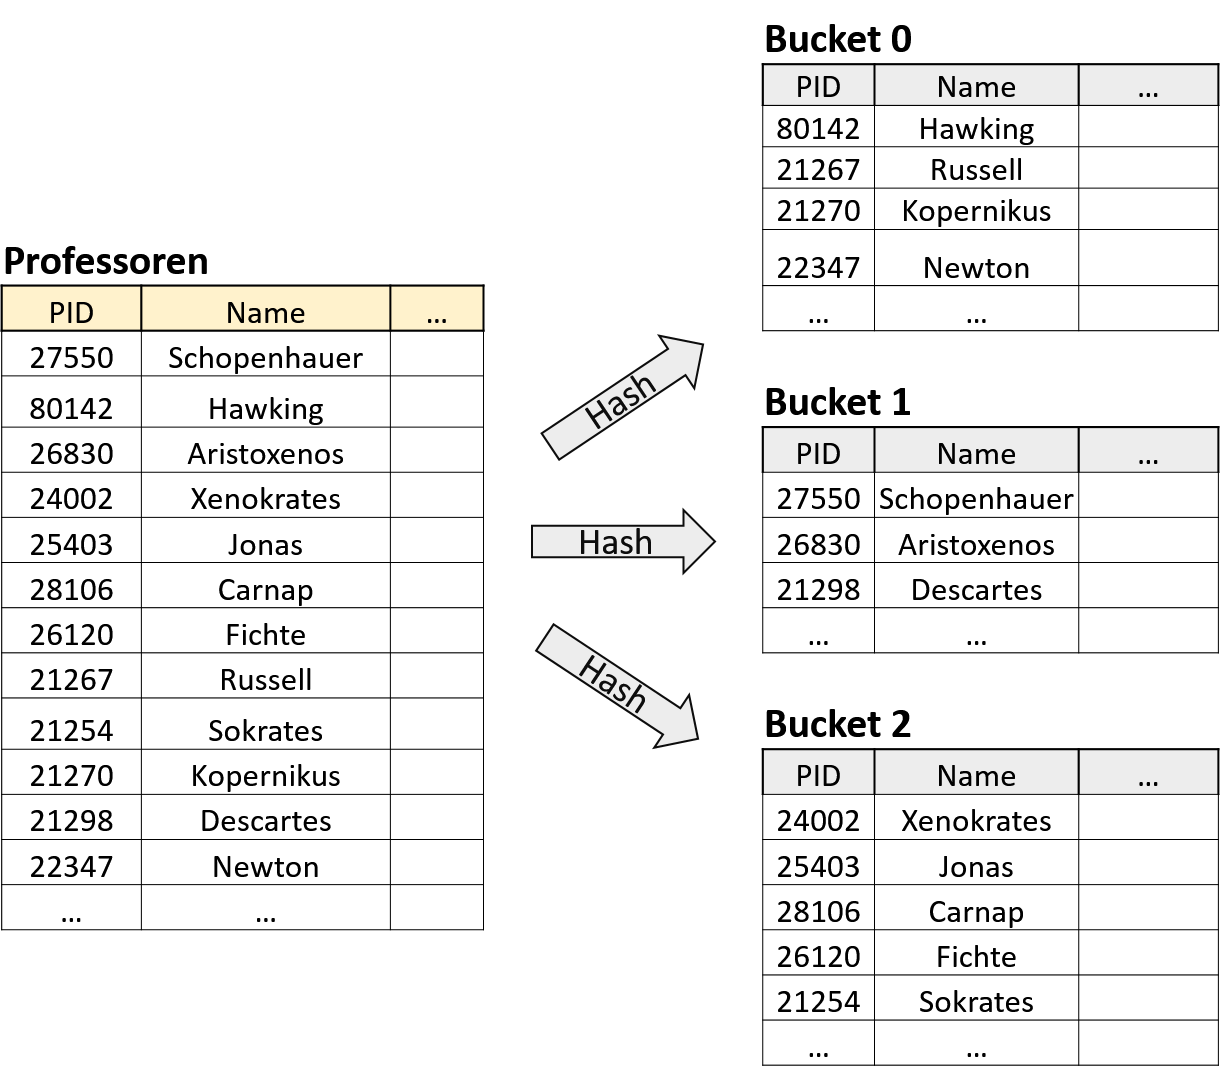
\includegraphics[scale=0.35, trim=0 0 0 4cm]{img/Hash-Bucket-0.png}
\\[-8pt]\caption{Mapping der Datens\"atze auf Buckets}
\end{figure}
\end{frame}

\begin{frame}
\frametitle{\insertsection}
\framesubtitle{\insertsubsection}
\structure{\textbf{Hash-Dateien}}\\[4pt]
\abs
Umsetzung: 
\begin{itemize}
	\item Einer Relation wird Speicherbereich von $p$ Buckets (Seiten) mit logischen Adressen $0, 1,\ldots, {p\text{\,--\,}1}$ zugeordnet. 
	\item Wertebereich (Dom\"ane) $S$ der Hash-Felder wird durch Hash-Funktion $h$ direkt auf eine Bucket-Adresse abgebildet. 
	$$h:S\to\{0, 1,\ldots, {p\text{\,--\,} 1}\},\quad s\mapsto h(s)\in\{0, 1,\ldots, {p\text{\,--\,} 1} \}$$
	In der Regel $\vert S\vert\gg p$, und somit $h$ \textbf{nicht} injektiv.
	\item Gebr\"auchlichste Art der Hash-Funktion: \emph{Division mit Rest} und meistens $p$ Primzahl.
	$$h(s) \equiv s\mod p$$
\end{itemize}		
\end{frame}

\begin{frame}
\frametitle{\insertsection}
\framesubtitle{\insertsubsection}
\structure{\textbf{Hash-Dateien}}\\[4pt]
Umsetzung: 
\begin{figure}
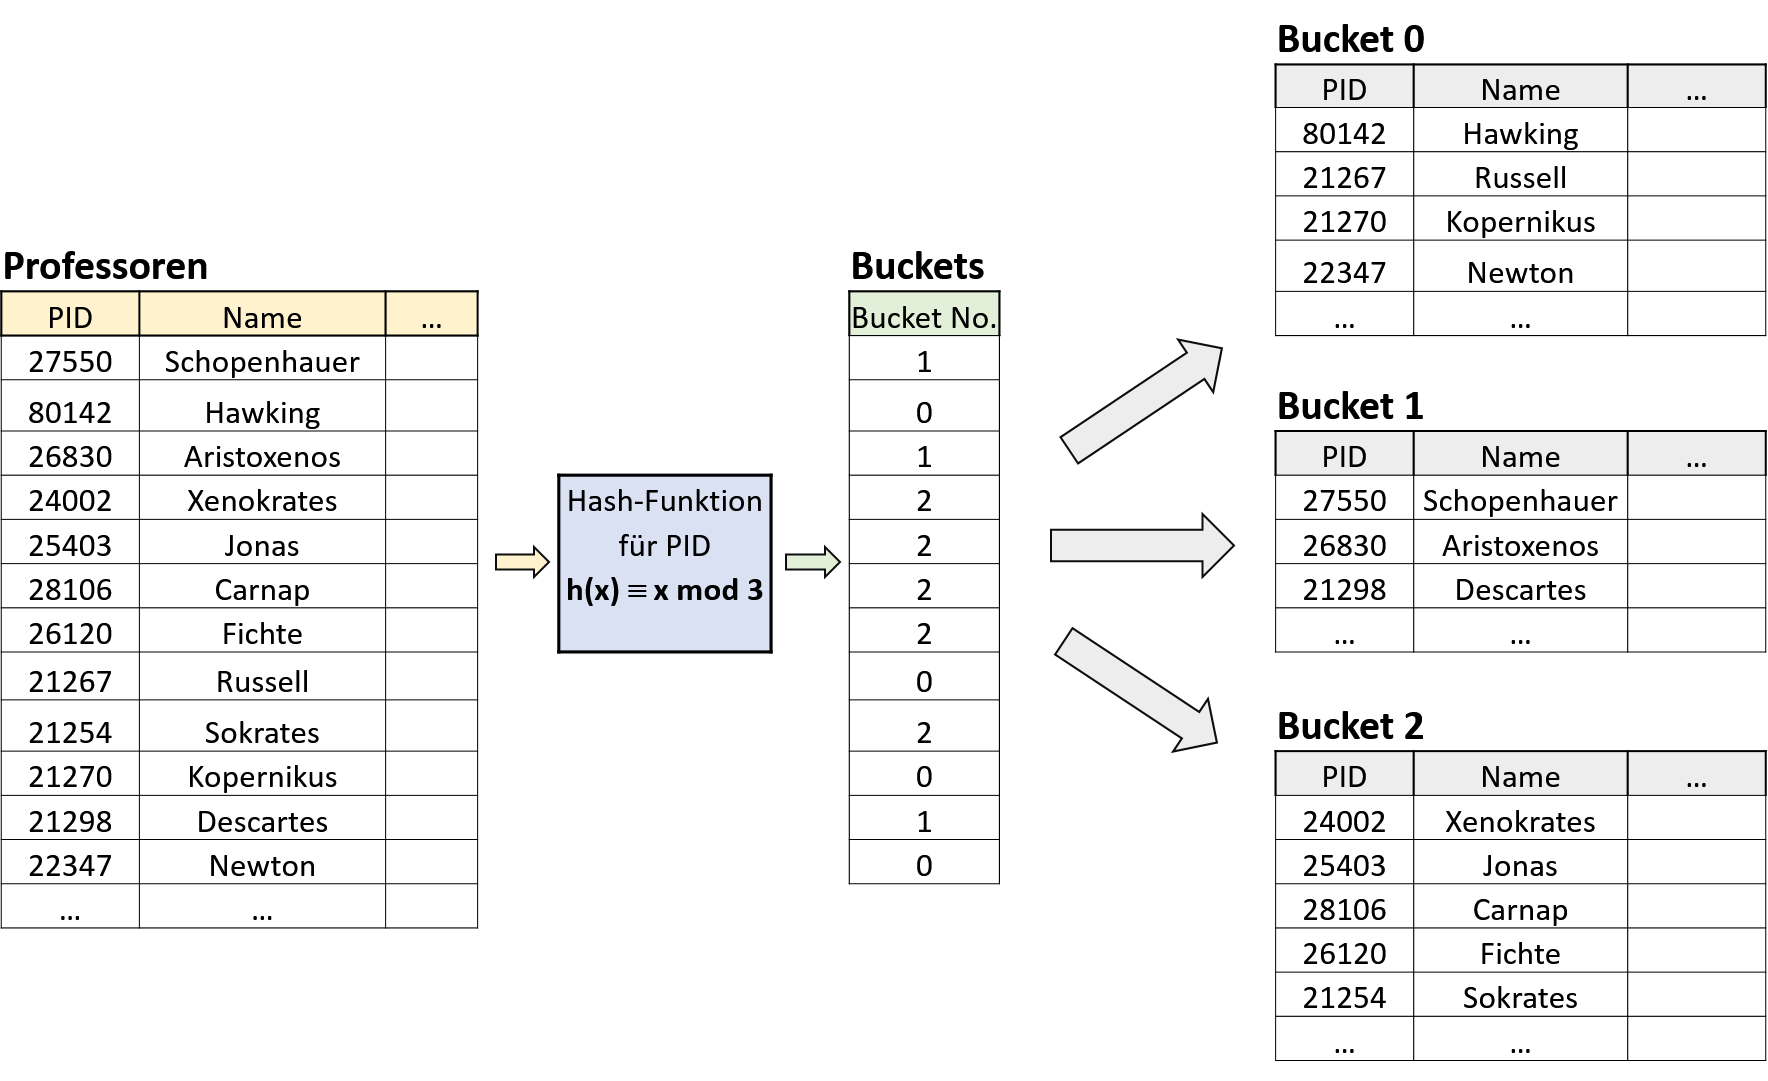
\includegraphics[scale=0.35, trim=0 0 0 4cm]{img/Hash-Bucket-1.png}
\\[-8pt]\caption{Mapping der Datens\"atze auf Buckets mit Hash-Funktion}
\end{figure}
\end{frame}

\begin{frame}
\frametitle{\insertsection}
\framesubtitle{\insertsubsection}
\structure{\textbf{Hash-Dateien}}\\[4pt]
\abs
Umsetzung Offenes Hashing: 
\begin{itemize}
	\item Ist beim Schreiben in der Seite des Bucket nicht genügend Platz, muss eine \"Uberlaufseite angelegt werden.
	\item Es wird ein Pointer in der vollen Seite auf die neue \"Uberlaufseite gespeichert.
	\item Eine \"Uberlaufseite kann wiederum \"uberlaufen, etc.
\end{itemize}		
\end{frame}

\begin{frame}
\frametitle{\insertsection}
\framesubtitle{\insertsubsection}
\structure{\textbf{Hash-Dateien}}\\[4pt]
Umsetzung: 
\begin{figure}
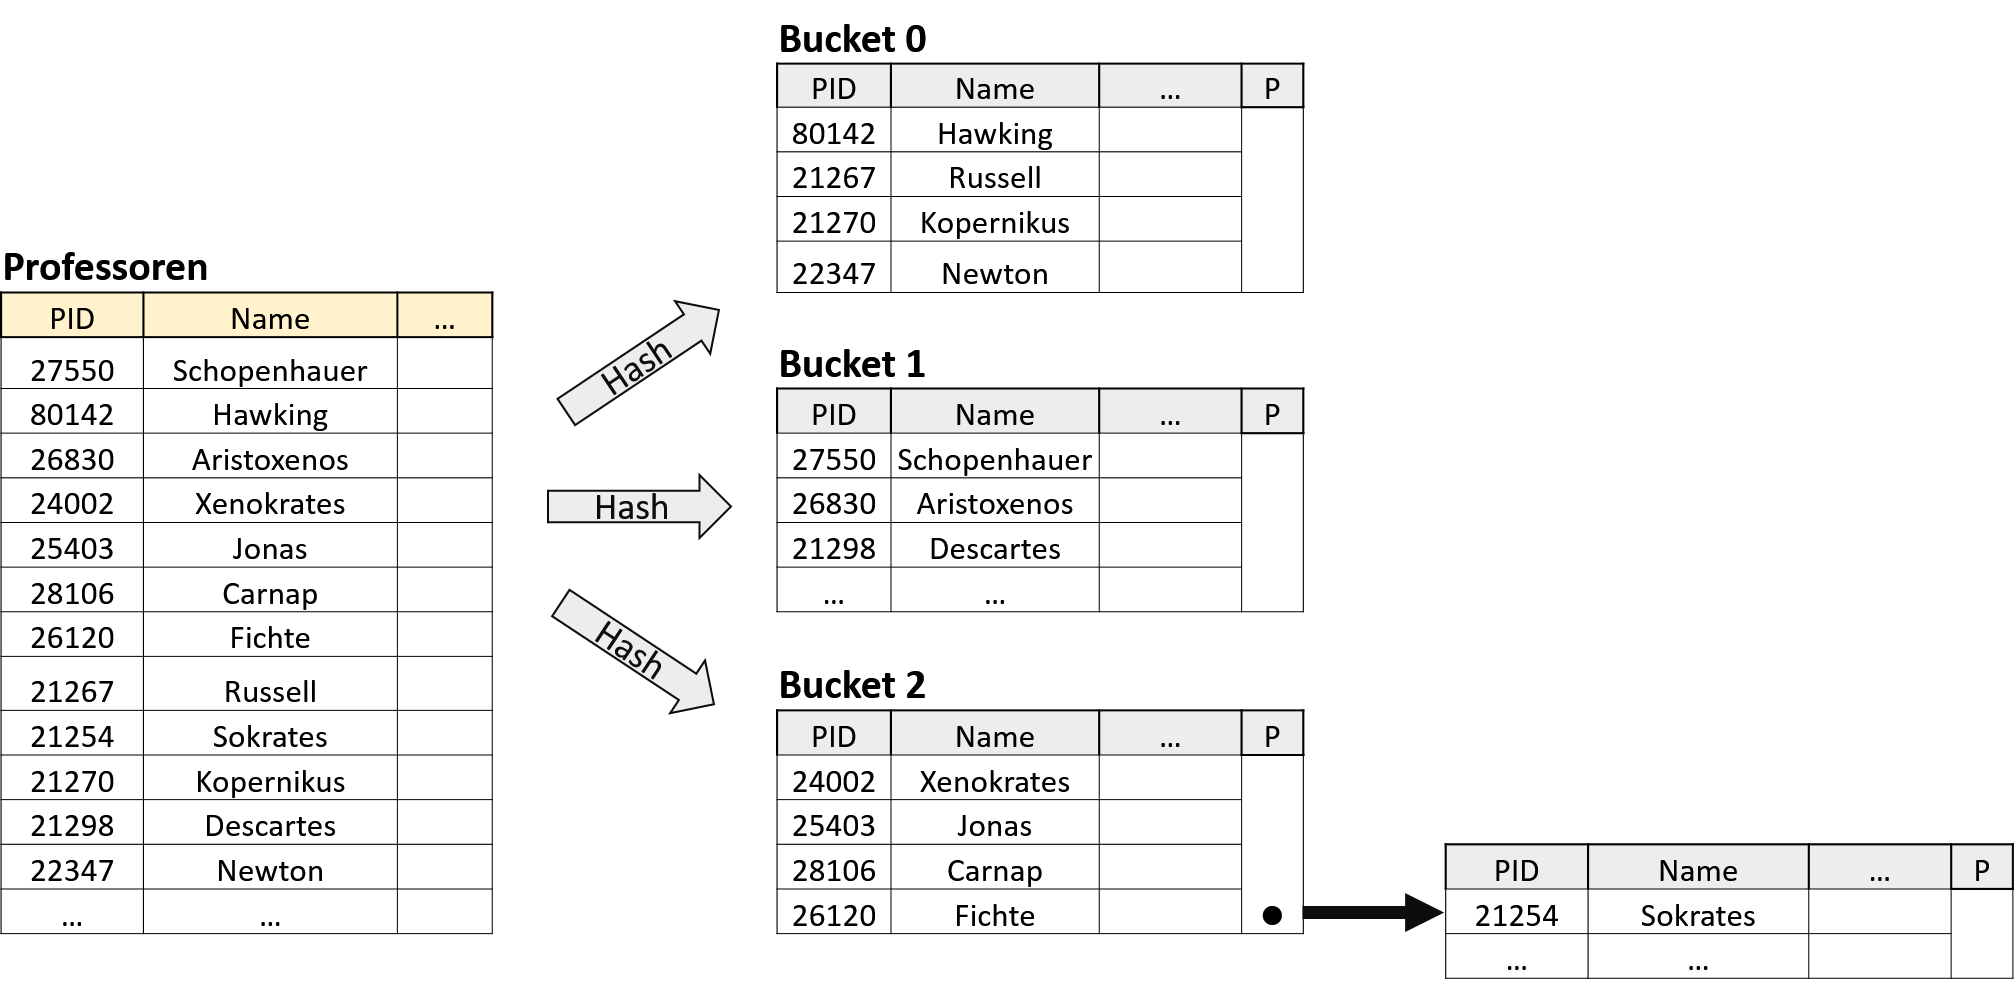
\includegraphics[scale=0.35, trim=0 0 0 4cm]{img/Hash-Bucket-3.png}
\\[-8pt]\caption{Mapping der Datens\"atze auf Buckets mit \"Uberlaufseite}
\end{figure}
\end{frame}

\begin{frame}
\frametitle{\insertsection}
\framesubtitle{\insertsubsection}
\structure{\textbf{Lesen in Hash-Dateien}}
\begin{itemize}
	\item Aus dem Feldwert wird m.~H.~der Hash-Funktion die Adresse der Seite und des Satzes direkt ermittelt. 
	\item Bei \"Uberl\"aufen muss die Kette linear abgearbeitet werden. 
	\item Ohne \"Uberlaufseiten kann auf jeden Datensatz in konstanter Zeit zugegriffen werden.
	\item Sehr schneller Zugriff.	
\end{itemize}
\end{frame}

\begin{frame}
\frametitle{\insertsection}
\framesubtitle{\insertsubsection}
\structure{\textbf{Schreiben in Hash-Dateien}}
\begin{itemize}
	\item Hash-Funktion liefert die Adresse des zugeordneten initialen Blocks.
	\item Bei \"Uberl\"aufen muss die Kette linear abgearbeitet werden. 
	\item Falls nicht gen\"ugend Platz vorhanden ist, wird eine neue \"Uberlaufseite angelegt, in die der Datensatz geschrieben wird.
\end{itemize}
\end{frame}

\begin{frame}
\frametitle{\insertsection}
\framesubtitle{\insertsubsection}
\structure{\textbf{L\"oschen in Hash-Dateien}}
\begin{itemize}
	\item Der betreffende Datensatz wird gesucht -- wie beim Lesen -- und aus dem Block eliminiert oder zum L\"oschen markiert. 
	\item Falls eine Überlaufseite leer wird, kann sie wieder freigegeben werden.
\end{itemize}
\end{frame}

% Speichereffizienz	HASH-Speicherstrukturen benötigen keine zusätzlichen Verwaltungsdaten. 
% Der Primärbereich muss ausreichend groß angelegt werden, damit neue Daten Platz finden und die Überlaufseiten nicht ausarten. 
% Bei veränderlichen Datenbeständen ist die Speichereffizienz niedrig.

\begin{frame}[t]
\framesubtitle{Gegenüberstellung: Heap -- Sortiert -- Hash}
{\small
	\begin{center}
		\begin{tabular}{|l|p{3cm}|p{3cm}|p{3cm}|}\hline
			& \textbf{Heap-Datei} & \textbf{Sortierte Datei} & \textbf{Hash-Datei}\\\hline
			Suchoperationen & Aufwändig. Alle S\"atze m\"ussen gelesen werden: $O(n)$, Durchschnitt $\frac{n}{2}$ 
			& Weniger aufwändig. Binäre Suche: $O(\log_2 n)$ & Nach Hash-Wert-Berechnung sehr schneller Zugriff\\\hline
			Einfügeoperationen & Schnell: Neuer Satz wird am Ende der Datei angeh\"angt 
			& Aufwändig. Dateien m\"ussen ggf.~umorganisiert werden 
			& Neuer Satz wird am Ende der Seite angeh\"angt. Ggf.~Erzeugen neuer \"Uberlaufseite\\\hline
			Löschoperationen & Aufwändig. Datensatz muss gesucht werden, Löschen hinterlässt Lücken, Reorganisation erforderlich 
			& M.~H.~von Sortierfeld günstiger. Ansonsten wie unsortierte Datei. Reorganisation erforderlich. 
			& \"Ahnlich wie bei Heap-Dateien\\\hline
			Sortierte Ausgabe & Sehr aufwändig & Sehr einfach & Sehr aufwändig \\\hline
		\end{tabular}
	\end{center}
}
\end{frame}

\section*{Übungsaufgaben}
\begin{frame}[t]
\frametitle{\insertsection}
\begin{alertblock}{Grundlagen der Datenspeicherung}
\begin{enumerate}
	\nowrite{ 
		\item Gegeben ist ein Datenschema \texttt{Kunde(\uline{KNR}, Vorname, Nachname, PLZ, Ort)}. Implementieren Sie ein Java-Programm, welches
		\begin{itemize}
			\item Eine Menge von Kundendatensätzen auf Festplatte speichern und wieder einlesen kann,
			\item einen Datensatz anhand der Kundennummer sucht,
			\item Datensätze anhand der PLZ sucht und
			\item Datensätze anhand des Nachnamens sucht, wobei Wildcards möglich sind (z.\,B. \texttt{Schmi*}).
		\end{itemize}
	}			
	\item Erläutern Sie, auf welche Weise Daten von der Festplatte in den Hauptspeicher übertragen werden.
	Gehen Sie in Ihren Erläuterungen nicht nur auf den Aufbau der Platte, sondern auch auf den Begriff der \textit{mittleren Zugriffszeit} ein.			
	\item Erl\"autern Sie den Begriff des \textit{Datensatzes} sowie den Begriff einer \textit{Datei}
	und erläutern Sie die drei aus der Vorlesung bekannten Speicherverfahren jeweils für Datens\"atze fester L\"angen und variable L\"angen 
	anhand eines Beispiels.			
\end{enumerate}
\end{alertblock}
\end{frame}

\begin{frame}[t]
\frametitle{\insertsection}	
\begin{alertblock}{Grundlagen der Datenspeicherung (forts.)}
\begin{enumerate}
\setcounter{enumi}{3}
\item Berechnen Sie den Blocking Factor für eine Blockgröße $b=1024$ und eine Satzlänge $r=327$.  
Wie viele Bl\"ocke werden für die Speicherung von 1000 S\"atzen ben\"otigt?
\item Durch die Abrundungsoperation bei der Berechnung von $\mathit{bfr}$ kann ggf.~das Ergebnis $\mathit{bfr}=0$ entstehen. 
Welche Aussage hat dieses Ergebnis und welche Konsequenz ergibt sich daraus?
\item In einer Heap-Datei wird der $i$-te Datensatz in den Festplattenblock
$$\left\lfloor{\frac{i}{\mathit{bfr}}}\right\rfloor,\quad \mathsf{Position~} (i \bmod \mathit{bfr})$$
gespeichert. Erl\"autern Sie, warum dieses Wissen im operativen Datenbankbetrieb faktisch nicht vorteilhaft ausgenutzt werden kann.
\end{enumerate}
\end{alertblock}
\end{frame}
